\section{Amazon S3}
\label{sec:Amazon S3}

Amazon S3 (Simple Storage Service) is an online file storage web service offered by Amazon Web Services. Amazon S3 provides storage through web services interfaces (REST, SOAP, and BitTorrent).Amazon launched S3, its first publicly available web service, in the United States in March 2006 and in Europe in November 2007 [25].
Amazon S3 is reported to store more than 2 trillion objects as of April 2013.[10] S3 uses include web hosting, image hosting, and storage for backup systems.  Amazon S3 provides an API (Application programming interface) for third-party developers. It describes various API operations, related request and response structures, and error codes.[38] Web services interface can be used to store and retrieve any amount of data, at any time, from any- where on the web. It gives any developer access to the same highly scalable, reliable, secure, fast, inexpensive infrastructure that Amazon uses to run its own global network of web sites. The service aims to maximize benefits of scale and to pass those benefits on to developers. Today, there are different kinds of file managers for Amazon S3. An effective solution for Amazon provides a user interface to Amazon S3 accounts, files and buckets, allowing to browse, create and delete files and buckets.

\subsection{Amazon S3 Multipart Upload}
\label{subsec:amazon_S3_multipart_upload_initiation}


In X-Learning platform the upload video use the Multipart upload API enables it to upload large objects quickly through the parallel upload of the n    parts of the object .
Multipart uploading is a three-step process: You initiate the upload, you upload the object parts, and after you have uploaded all the parts, you complete the multipart upload. Upon receiving the complete multipart upload request, Amazon S3 constructs the object from the uploaded parts, and you can then access the object just as you would any other object in your bucket.
You can list of all your in-progress multipart uploads or get a list of the parts that you have uploaded for a specific multipart upload. Each of these operations is explained in this section.


\begin{figure}[htb] %  figure placement: here, top, bottom
 \centering
 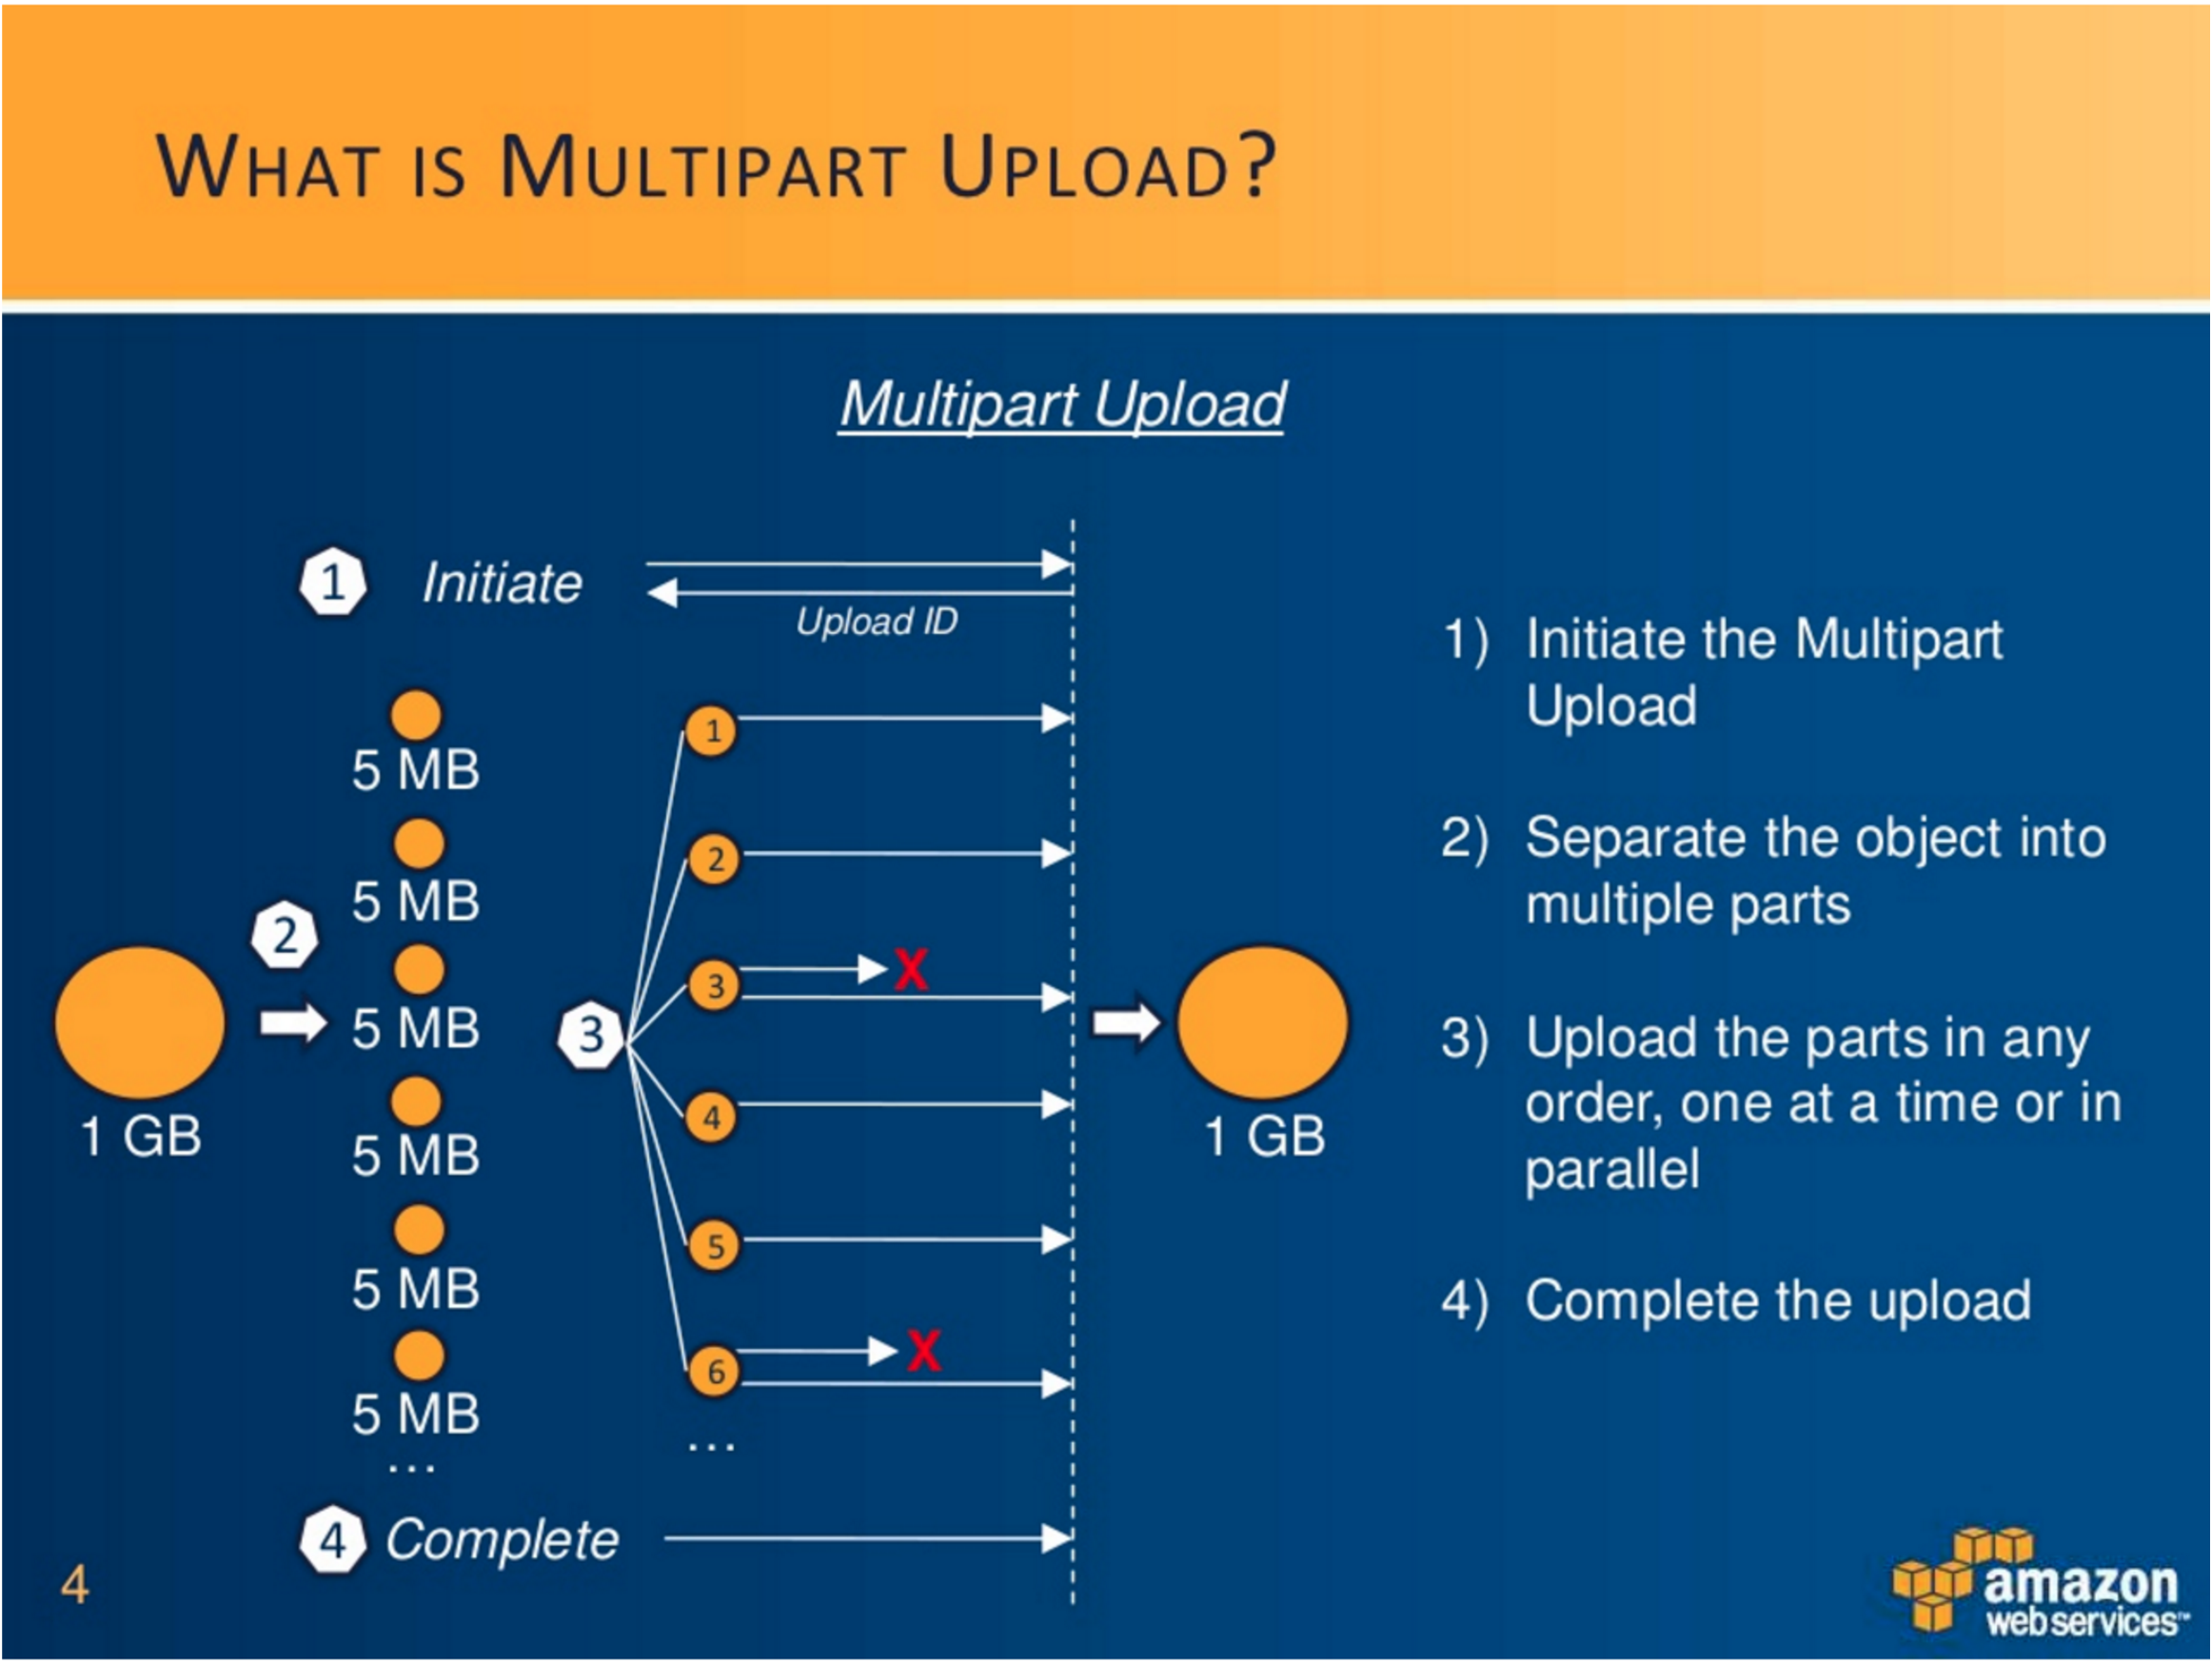
\includegraphics[width=1.0\linewidth]{images/chapter2/multipart_upload.png}\hfill
 \caption[Multi part Upload]{The MultiPart Upload}
 \label{fig:fourV}
\end{figure}

\subsection{Amazon S3 Multipart Upload Initiation}
\label{subsec:amazon_S3_multipart_upload_initiation}

When you send a request to initiate a multipart upload, Amazon S3 returns a response with an upload ID, which is a unique identifier for your multipart upload. You must include this upload ID whenever you upload parts, list the parts, complete an upload, or abort an upload. If you want to provide any metadata describing the object being uploaded, you must provide it in the request to initiate multipart upload.


\subsection{Parts Upload}
\label{subsec:parts_upload}

When uploading a part, in addition to the upload ID, you must specify a part number. You can choose any part number between 1 and 10,000. A part number uniquely identifies a part and its position in the object you are uploading. If you upload a new part using the same part number as a previously uploaded part, the previously uploaded part is overwritten. Whenever you upload a part, Amazon S3 returns an ETag header in its response. For each part upload, you must record the part number and the ETag value. You need to include these values in the subsequent request to complete the multipart upload.
After you upload one or more parts, you must either complete or abort multipart upload in order to stop getting charged for storage of the uploaded parts. 


\subsection{Multipart Upload Completion (or Abort)}
\label{subsec:multipart_upload_completion}

When you complete a multipart upload, Amazon S3 creates an object by concatenating parts in ascending order based on the part number. If any object metadata was provided in the initiate multipart upload request, Amazon S3 associates that metadata with the object. After a successful complete request, the parts no longer exist. Your complete multipart upload request must include the upload ID and a list of both part numbers and corresponding ETag values. Amazon S3 response includes an ETag that uniquely identifies the combined object data. This ETag will not necessarily be an MD5 hash of the object data. You can optionally abort the multipart upload. After aborting a multipart upload, you cannot upload any part using that upload ID again. All storage that any parts from the aborted multipart upload consumed is then freed. If any part uploads were in-progress, they can still succeed or fail even after you aborted. To free all storage consumed by all parts, you must abort a multipart upload only after all part uploads have completed.

\begin{figure}[htb] %  figure placement: here, top, bottom
 \centering
 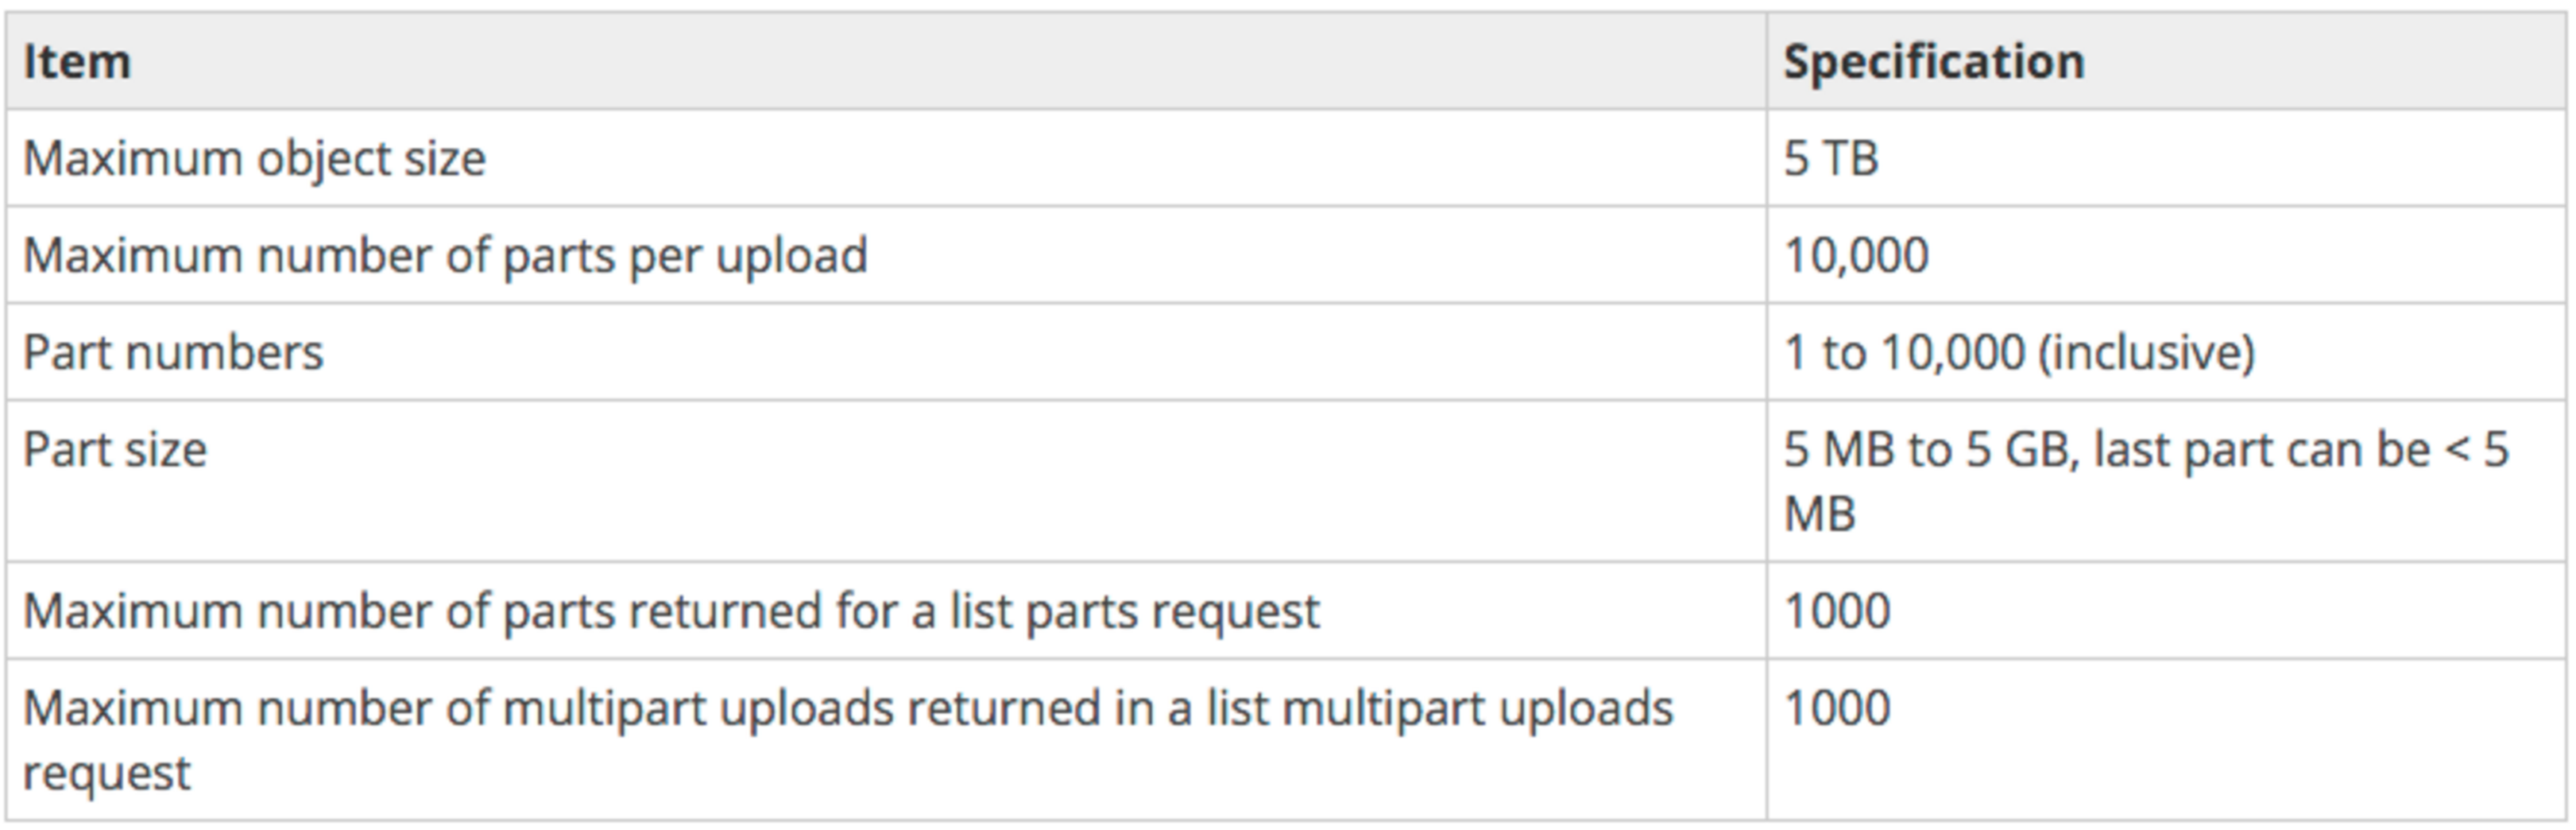
\includegraphics[width=1.0\linewidth]{images/chapter2/multi_part_info.png}\hfill
 \caption[Multi part Upload info]{The MultiPart Upload info}
 \label{fig:fourV}
\end{figure}
